
We have implemented a fully functional program that works from user putting in input to writing the output.

We utilized the following technologies:

\begin{itemize}
\item \textbf{Java}\\
As for the programming language, Java has been chosen for numerous reasons.
\begin{itemize}
\item Java is an object-oriented language which incredibly goes with the modeling principles of this paper.
\item We wanted a high-level language to be able to fully separate our program from the low-level parts so that the models are not dependent on architecture.
\item With Java, we are able to use Maven for effortless dependency management.
\item Robustness and security are benefits implied directly by the language's design. Java puts significant emphasis on early checking for possible errors and so compilers are able to detect many problems that would first show up during execution time in other languages.
\item Much of the code we would write has already been implemented by someone and we can just use it in form of libraries.
\item Multithreading is easily achievable in comparison with other languages and provides the ability to simultaneously perform tasks such as computing, serving GUI, communicating with a database, managing resources, and garbage collecting.
\end{itemize}
\item \textbf{Git}\\
One of the most important benefits of a version control system is traceability, providing with the ability to explore history. We use Git since it is one of the most common version control systems, offers a great tool-set and vast majority of open source software uses it because of the community using it. Another advantage of employing Git is the possibility to host the code on GitHub.
\item \textbf{Maven}\\
Maven is a software project management and comprehension tool. It can manage a project's build, dependencies, reporting and documentation from a central piece of information contained in one file. Once you introduce Maven into your project, building it and including project libraries can never be simpler anymore.
\item \textbf{MySQL database}\\
We use a database for storing and retrieving various values, e.g. coordinates of the cities, time zone data, average temperatures, sun declination values etc.
\end{itemize}

Figure \ref{uml} is an UML diagram presenting classes of the program that have the most important role.

\begin{figure}[ht]
    \centering
        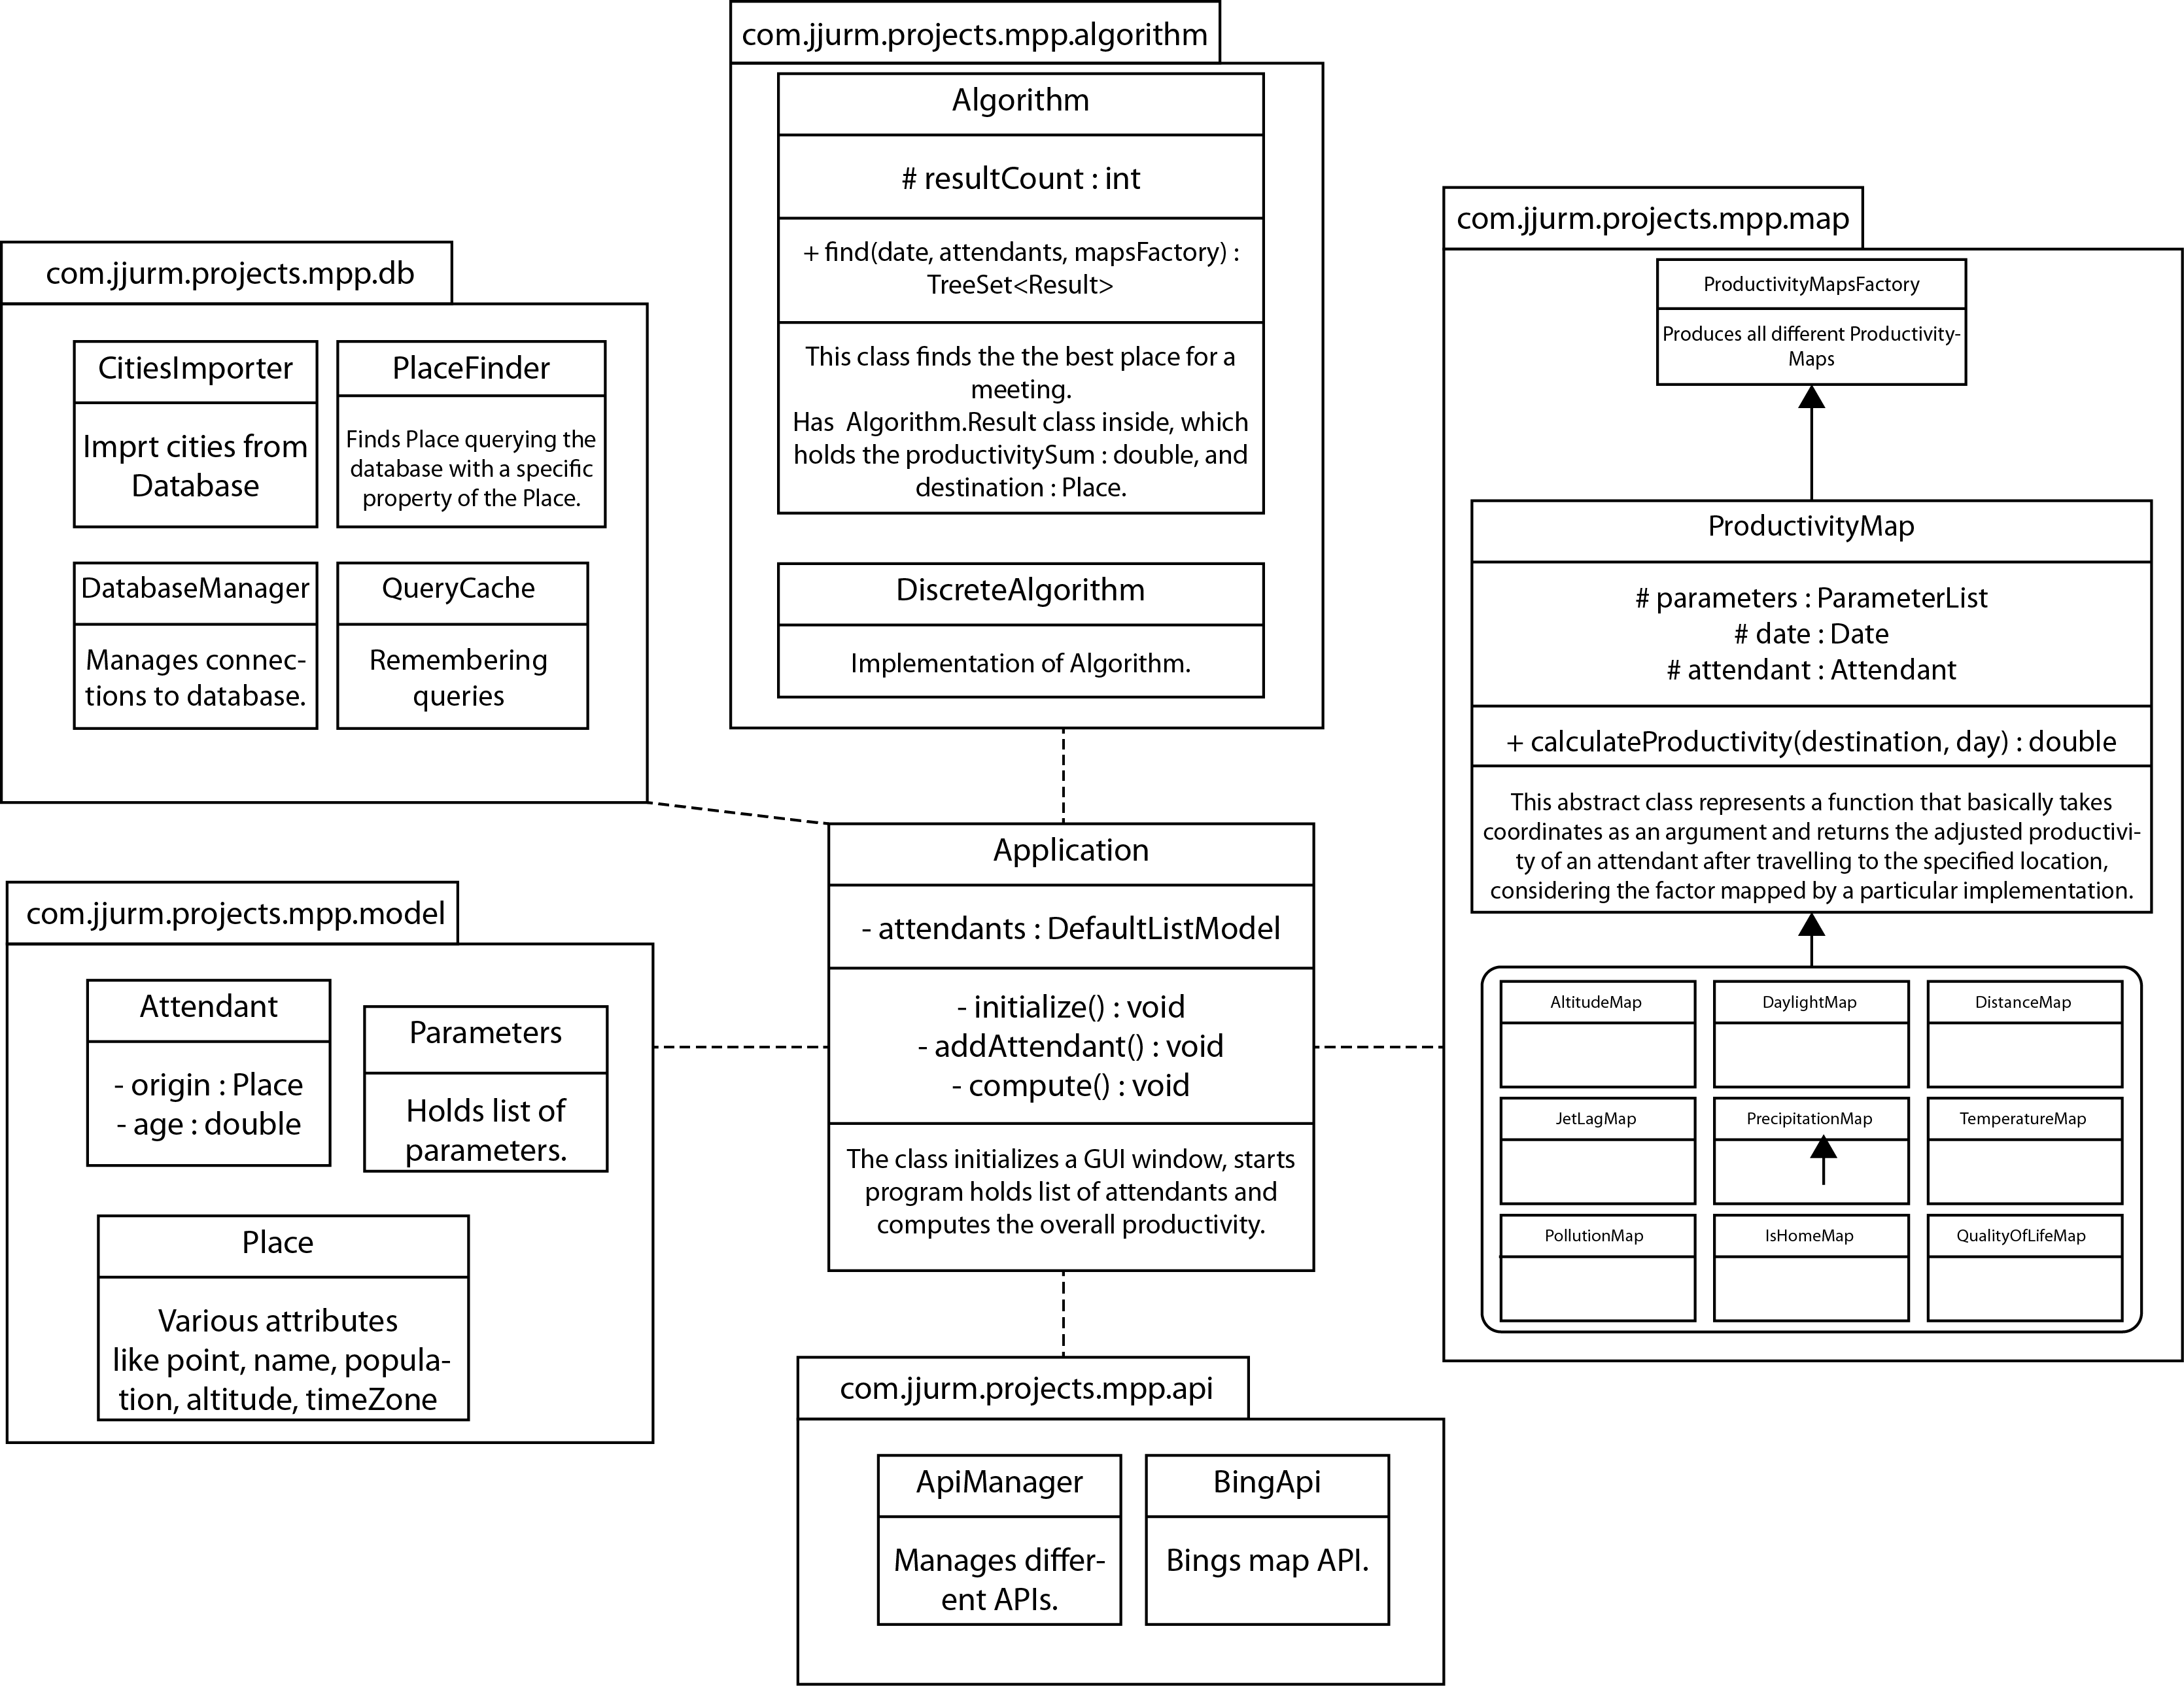
\includegraphics[width=\textwidth]{mpp.png}
    \caption{UML diagram of important classes}
    \label{uml}
\end{figure}

Our code is publicly available at the following address:\\ \url{https://github.com/jjurm/meeting-point-planner}

The hash of the final commit is \texttt{d6b4937bd784a0977ea1b6808f83e7d98bf67576}

You can find the full listing of our code in Appendix \ref{appendix:code}.